%% ----------------------------------------------------------------------
%% START OF FILE
%% ----------------------------------------------------------------------

\chapter{相关技术简介}
\label{cha:related_work}

\section{存储介质简介}

\subsection{机械硬盘(HDD)}
机械硬盘\cite{hdd2009}(HDD,Hard Disk Driver)是个人计算机中一种应用最为广泛的非易失性的存储设备,使用覆盖有氧化铁的坚硬旋转盘片为存储介质。机械硬盘内部的物理结构分为磁盘、电动机、悬臂和主控芯片几部分。磁盘盘面以磁道、柱面和扇区的方式组织表面空间。由电动机带动盘片旋转,副电动机带动悬臂上的磁头移动到碟片表面的某个位置。磁头悬浮在磁盘的正反两面上,磁盘旋转时磁头会在盘片表画出一个与磁盘同心的圆形轨道(称磁道或柱面)。此时,磁头内部的磁感线圈感应磁盘上的磁铁极性,通过时间间隔定位扇区,通过电流读取、写入数据内容到当前磁头所处的扇区。

通过磁化盘片表面上磁铁单元的极性,机械硬盘在平整的磁性表面上存储最基础的01比特数据。离磁性表面很近的读写磁头利用磁铁单元对电流的电感效应完成读写。盘片的两个存储面上各存在一个磁头负责读写,所有磁头的水平运用方向保持一致,磁头的移动方向由磁头控制器所负责。磁头只能沿盘片半径在水平方向上运动,结合电机带动盘片的高速旋转,磁头可以定位到盘片正反面上的任意位置进行记录数据的读写操作。

\begin{figure}[H]
\centering
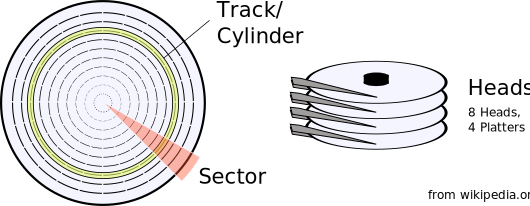
\includegraphics[width=0.6\linewidth]{./graph/hdd-struct}
\caption{机械硬盘结构}
\label{fig:hdd-struct}
\end{figure}

\begin{itemize}
\item 磁道
\\当磁头保持在某个位置上时,磁盘旋转,磁头会在磁盘表面画出一个与磁盘同心的圆圈,我们称圆圈的轨迹叫做磁道(Track)。
\item 柱面
\\磁盘中通常存在一或多个盘片,竖直上的不同盘片、水平上处于同一半径的多个圆形磁道组成的一个圆柱面(Cylinder)。
\item 扇区
\\每个圆形磁道按照角度又被等分为若干个弧段,每个弧段是硬盘上的一个扇区(Sector)。一般称磁盘的首个扇区为引导扇区。
\end{itemize}

一般以RPM(每分钟的转动数)为单位描述机械硬盘盘片旋转速度,存在5400、7200、10000、15000几种规格。电机带动盘片转速越高,数据读写速率愈快,但噪音和发热量也上升明显。7200转属于最常见的磁盘转速。

机械硬盘内部的盘片、磁头机械结构决定了机械硬盘擅长于顺序读写,随机读写性能较差。

\subsection{固态硬盘(SSD)}
固态硬盘\cite{ssd2009}(SSD,Solid State Driver)作为一种存储设备,既可以基于永久性存储介质,如Flash闪存,也可以基于非永久性存储介质,如同步动态随机存取存储器(SDRAM)。设计固态硬盘的初衷是为了替代传统机械硬盘。固态硬盘内部已没有了像机械硬盘那样可以旋转的盘片结构,但是为了兼容人们对存储设备的命名习惯,固态存储器仍被称作硬盘。根据上面提到的所基于的两种存储介质,固态硬盘分为易失性和非易失性两类。

\begin{enumerate}
\item 基于易失性记忆体的固态硬盘

使用易失性记忆体作为存储介质的固态硬盘,通常用于临时存放数据。易失性记忆体需要外界电力维持其内部的记忆功能,因此为了防止断电时的数据丢失,一般需要配合电池进行不间断供电。以SDRAM为代表的易失性存储介质,具有访问速度快(接近内存速度)、使用寿命长的优点。利用速度上的优点,软件程序可将需要访问的数据从机械硬盘转存到固态硬盘中,以此减少机械硬盘电机的启停延迟、磁头的寻道延迟对数据访问速度的影响。

此外,基于易失性记忆体的固态硬盘还可用于应急备份。这类固态硬盘一般会使用电池提供备用电力,即使遭遇意外停电,固态硬盘还可短暂利用电池电力,将数据转移到非易失存储设备。恢复电力后,再将数据从非易失存储设备转移过来。

\item 基于非易失性记忆体的固态硬盘

基于非易失性记忆体的固态硬盘在外观上和机械硬盘已经没有什么区别。以NVRAM为代表的非易失性存储介质的数据存取速度,介于易失性介质SDRAM和机械硬盘之间。相比于易失性介质,非易失性介质数据一经写入,便无需额外电力以维持其存储能力,不必考虑断电的影响使其更有潜力替代常规硬盘。

每块固态硬盘内部都会存在多个存储颗粒,每个存储颗粒中有非常多的存储单元储存数据。目前,市面上存在三种主流的制造固态硬盘存储单元的NVRAM颗粒,分別是多层式储存颗粒(MLC,Multi Level Cell)、单层式储存颗粒(SLC,Single Level Cell)和三层式储存颗粒(TLC,Triple Level Cell)。SLC、MLC和TLC三者的区别是存储颗粒内部单个存储单元所能存储的状态个数:SLC一种,MLC两种,TLC三种。这三者的读写速度几乎没有差别。TLC颗粒主要在企业级固态硬盘中使用,但是成本很高,使用MLC和TLC颗粒制造的固态硬盘的成本低,但是寿命较短。

由于存储颗粒内部每个存储单元的写入次数是有限的,存储颗粒的最大写入次数便是存储颗粒的使用寿命。固态硬盘控制器通常会把写操作平均分配到存储颗粒内部的每个存储单元上,再通过映射表的方式定位数据的实际存储位置。工业界使用P/E cycle这一参数标准衡量固态硬盘的使用寿命,一个P/E cycle代表了固态硬盘内所有的存储颗粒被写入一次。固态硬盘的P/E cycle参数体现了硬盘内部存储颗粒可写入次数的峰值,P/E cycle越大固态硬盘的使用寿命越长。

\begin{table}[htb]
\centering
\caption{SLC、MLC和TLC的寿命和价格比较}
\begin{tabular}{|c|c|c|c|}
\hline  & SLC NAND Flash & MLC NAND Flash & TLC NAND Flash \\
\hline P/E Cycles & 100,000 & 10,000 & 4,000 \\
\hline Cell type & 1bit/cell & 2bit/cell & 3bit/cell \\
\hline Price (USD/GB) & 5 & 1.4 & 1 \\
\hline
\end{tabular}
\label{tab:slc-mlc-tlc-compare}
\end{table}

从表\ref{tab:slc-mlc-tlc-compare}可以看出,存储颗的粒密度从SLC到TLC逐渐增大,而P/E cycle逐渐减少。SLC颗粒常被用于生产企业级的固态硬盘,而MLC颗粒和TLC颗粒则较多的出现于桌面计算机的固态硬盘中。虽然TLC颗粒的P/E cycle与SLC颗粒存在将近两个数量级的差距,但实际应用情况表明,使用TLC存储颗粒的固态硬盘完全可以满足桌面计算机的使用寿命要求。

尽管相比较于机械硬盘,固态硬盘有着如此多的优势,但使用非易失性颗粒的固态硬盘并不是不存在缺点。在硬盘剩余空闲空间不多时,极有可能出现严重影响写入性能的Write cliff现象。Write cliff现象出现在当所有存储颗粒的空闲页都已经被初始化写入,新的写请求无法一次性得到足够的空闲页以完成写入操作的情况下。此时,固态硬盘控制器必须要擦除某些未写满的存储页面再进行写操作:控制器会将未写满存储页面的原有数据拷贝到临时空间,再进擦除;将原有数据与新数据进行合并,写入到擦除后的存储页面。拷贝原有数据到临时空间消耗的时间是Write cliff出现的主要原因。

固态硬盘厂商为了减少Write cliff对性能的影响,特别加入了特别针对固态硬盘删除数据的TRIM指令。当需要删除文件时,可通过TRIM指令会告知固态硬盘被删除文件的位置,固态硬盘控制器会将对应的存储块标记为空闲状态。这样,就能在一定程度上保证总是存在空闲页,从而降低Write cliff现象出现的概率。TRIM指令的出现,很大程度上提升了固态硬盘的性能、延长了固态硬盘的寿命,但当空闲页面无法满足写请求时,仍然需要擦除未写满的存储页面。可以得出的结论是,TRIM命令只能推迟而无法避免Write cliff现象的出现。
\end{enumerate}

\subsection{机械硬盘与固态硬盘的比较}
固态硬盘出现的目的是替代传统的机械硬盘,但是机械硬盘相较于固态硬盘的某些优势使得固态硬盘不可能在短期内动摇机械硬盘的统治地位。两者之间的差距可从以下几个方面进行比较。

\begin{enumerate}
\item 安全性
\\机械硬盘内部的盘片、电机等机械构造决定了在发生碰撞和震动时,磁头和盘片的接触往往会造成机械硬盘的损坏,从而导致数据的丢失。固态硬盘内部使用的缓存芯片几乎不受碰撞和震动的物理影响。
\item 性能
\\无论是启动速度还是IO性能,固态硬盘都有着非常明显的优势。造成这种优势的主要原因是固态硬盘内部不是机械结构,不需要寻道以定位数据。传统的机械硬盘则需要在指令接受后开始寻道。因此固态硬盘在读写速度,尤其是随机读写上,较普通机械硬盘存在很大优势。
\item 价格
\\2012年的统计数据表明,固态硬盘的价格是0.67美元/GB,传统的机械硬盘的价格是0.09美元/GB,固态硬盘价格是机械硬盘的7倍多。造成价格悬殊的主要因素是机械硬盘发展较早,技术相对成熟;固态硬盘制造工艺则有待提高。固态硬盘的高昂价格会让很多用户在购买前三思,他们更倾向于暂失固态硬盘的诸多优势而选择性价比更高的机械硬盘。
\item 容量
\\海量数据时代的到来和用户对更高品质交互体验的追求,带来了日益增长的数据存储空间需求。大容量固态硬盘不仅非常稀少且价格昂贵,主流的固态硬盘一般都为128GB、256GB或512GB的存储空间。实际情况是,1TB的机械硬盘都已难以满足桌面电脑的需求,更不用说数据量巨大的企业级用户。
\item 耗电量
\\机械硬盘使用电机驱动盘片旋转和磁头移动,耗电量约为固态硬盘的3倍多。对于移动设备来讲,耗电量的多少是衡量电池所能支持待机时间的关键。同样的,在存在上百个磁盘阵列的数据中心部署固态硬盘,可以节约大量电能,从而减少电费支出。但基于易失性存储器的固态硬盘需要不间断供电,否则可能会导致数据丢失。
\item 重量和形状
\\由于不存在机械硬件的磁盘、电机等部件,固态硬盘的平均重量仅仅有70-85克,而机械硬盘则可达到650-800克,这一优势可使便携的移动设备同时搭载几个固态硬盘成为可能。同时,完全半导体化的固态硬盘内部结构,使其在物理上无样式、结构的限制,可根据实际需求改变固态硬盘的接口、形状。
\item 工作温度
\\由于固态硬盘本身的功耗就不高,所以其在工作过程中产热也相对较低。而机械硬盘每分钟5000转以上的转速,盘片和空气的摩擦以及不同机械部件之间的摩擦所产生的热量远高于固态硬盘,温度太高很容易使机械硬盘的脱离正常工作状态。固态硬盘不但本身产生的热量少,而且能够工作在更宽泛的温度范围内。
\item 噪音
\\ 得益于使用闪存芯片不存在机械构件,固态硬盘不会产生噪音。而机械硬盘运行时则会产生一定的噪音。尤其是存储中心大规模的磁盘阵列所产生的巨大噪音,更是需要设立专门的机房进行存放。
\end{enumerate}

\section{存储系统缓存技术}
\label{sec:storage_cache_tech}

尽管自二十世纪九十年代以来,计算机硬件技术的发展带来了磁盘存储密度每半年到一年一倍的提升,但没有相应的技术能够以同样的速度缩短存储介质的访问时间。缓存技术\cite{cache2011}作为一种减少IO子系统的响应时间、增加系统吞吐量的解决方案,已被广泛应用于存储子系统中。

\subsection{缓存的特点}
保存了主存储器中少部分数据复制品的缓存,其访问速度远高于主存储器。如果使用缓存中的数据就可以满足某个访问主存储器的请求,则称缓存命中了一次。

由于缓存中保存的是主存储器中的部分数据,因此会出现找不到所需数据而无法命中的情况,此时则需要访问主存储器才能获得数据。如果这种情况发生的比例超过一定数值,缓存对系统性能的提升就无法得到保证。不命中情况下获得的主存储器数据被用来更新缓存内的数据内容,以便下次访问不再需要到主存储器中获取数据。由于被频繁访问的数据并不是一成不变的,因此需要缓存页面替换算法不定期的更新缓存内的数据,这样才能保证缓存中的数据是被访问最频繁的,命中率才有保证。

\subsection{缓存的工作原理}
为了形象说明缓存系统的工作原理,本小节会以CPU访问内存中的数据为例进行说明。绝大多数CPU中都集成了一或多级的高速缓存以缩短访问内存的时间。

CPU执行过程中需要内存中的某个数据时,首先会从高速缓存中查找,如果能够找到,则无需访问内存CPU即可进行处理,几乎没相应延迟;如果没有找到,就只能从响应延迟高的内存中读取后传送给CPU进行处理,同时,将获得的数据块调入高速缓存中。更新缓存中的数据一定程度上可以增加数据在缓存中进行的概率,减少内存的访问。正是这一机制使大多数CPU可达到90\%左右的高速缓存命中率,只有10\%的访问操作需要真正读取内存。减少了需要CPU直接访问内存的次数,也就使得CPU几乎无需等待,就能获得所需数据。一般来说,CPU需要数据时总是先查缓存、后访内存。

\subsection{缓存数据替换算法}
缓存系统运行过程中,需要对存储设备上的数据按照请求的频率进行冷热程度的划分。性能较高的存储设备储存经常访问的热数据,存储在性能较低的设备储存不经常访问的冷数据,以达到区分对待冷热数据的效果。缓存数据替换算法在缓存系统运行过程中,通过识别出的冷热数据,不断移动和更新缓存中数据,尽可能保证热数据存储在性能较高的存储设备,以达到提升缓存命中率和系统性能的目的。所以,从本质上讲,缓存数据替换算法就是数据的热度识别和存储组织管理算法。

从缓存提升系统性能的原理不难得出,区分冷热数据的准确程度直接影响了缓存系统的IO性能。学术上已经有很多关于区分冷热数据的算法研究成果。根据缓存空间组织的粒度,缓存数据替换算法可以分为两类,不同类型算法的识别的准确程度和计算复杂度会有不同。下面将逐一进行介绍。

\begin{enumerate}
\item 数据块级

数据块是最小的数据空间划分单位,通过数据块识别冷热数据需要将主存储空间和缓存空间按照相同大小的数据块进行划分。将数据块看作是统计冷热程度的最小单位,通过统计每个数据块的访问计数,将标记访问计数大的数据块为热数据块。固态硬盘内部的设计中,数据块的热点识别还可用于固态硬盘的损耗平衡:通过一定的映射策略,将写操作平均分配到所有的存储块。

数据块级的冷热数据识别的优势在于,它可以在文件系统无关的存储层面精确地定位出所有的热数据块,同时又不必在考虑例如存储空间组织结构、文件系统等宏观的信息,从而简化了识别冷热数据的计算过程,保证了系统性能受计算复杂度的影响尽可能小。

\item 文件级

文件级别的冷热数据划分\cite{linlin2011}是另一种缓存数据替换算法用到的判定方法。这种以文件作为热度统计的最小单位的方法,为每个文件开辟专门用于保存访问计数的元数据区域。所有的文件访问操作都会对改变元数据区域中的访问计数值。文件级别的冷热数据划分可以从文件类型、文件大小、同时打开文件的进程数目等多种宏观层面指标进行综合判别,提升判别的准确程度。

相比于数据块级别,文件级的判定更能够节省统计数据的存储空间,进而减少缓存系统额外的缓存空间消耗。而且还可以将随机性因素加入文件访问的识别过程,更好的区分冷热数据文件。
\end{enumerate}

\subsection{缓存系统存在的目的}
缓存系统的存在通常是为了达到三个目标:
\begin{itemize}
\item 减少交互的通讯量:缓存数据能最小化在进程和网络间传输的数据量。
\item 降低系统中的处理量:记录处理结果,避免数据的重复处理。
\item 降低主存储器的访问次数:如操作系统内核在内存中缓存的机械硬盘数据。
\end{itemize}

在评估一个缓存系统的好坏时,一般会从性能、稳定性和可用性三个方面进行:
\begin{itemize}
\item 性能:定量分析访存请求在缓存中的命中率和带来的延迟的缩短。
\item 稳定性:缓存算法本身是否稳定性,对于意外情况(如掉电),能否保证数据完整。
\item 可用性:缓存系统对应用是透明的,应用感受到的,仅仅是飞快的响应速度和良好的可用性。
\end{itemize}

\section{混合存储系统}
\label{sec:hybrid_storage}

只要数据的处理速度和存储介质的访问速度、不同类型存储介质的访问速度仍然保持较大的差距,学术界和工业界就不会停止研究和探索利用不同速度的存储器件,搭建混合存储系统\cite{zhuqing2013hybrid}以提高系统的性能、容量和可靠性等指标。通过近二十年的研究,科学家和工程师们已经获得了众多的研究成果。

\subsection{基于DRAM与机械硬盘的混合存储}

使用DRAM为机械硬盘缓存数据\cite{sdramcache2002},毫无疑问,是提高机械硬盘性能的重要手段之一。几乎所有操作系统在设计磁盘驱动程序时,都会优先考虑使用DRAM缓存机械硬盘的数据。硬盘制造商在制造硬盘时,同样会在硬盘控制器中加入8-16MB的DRAM芯片。利用数据的空间局部性原理,硬盘控制器在处理IO请求时读取的数据量会略大于请求的数据量,并在DRAM进行缓存。处于硬盘控制器中的DRAM缓存对于软件来说是透明的,磁盘驱动程序不必关心控制器缓存的运行情况。

由于DRAM的易失性限制,通常只用使用DRAM作为读缓存提高机械硬盘的性能,对写性能几乎起不到提高的效果。如果也缓存写操作,为了避免写入机械硬盘的脏数据由于掉电而丢失,磁盘控制器或是驱动程序就必须将脏数据持续的从DRAM写回到机械硬盘,以降低数据丢失的风险。因此,使用DRAM缓存面临着数据可靠性和读写性能间的两难选择,缓存越大性能提升越明显,停留在缓存中的脏数据丢失的可能性也就越大。基于以上原因的考虑,任何缓存系统都会限制缓存中脏数据的停留时间和所占比例。

\subsection{基于NVRAM与机械硬盘的混合存储}

NVRAM存储数据非易失性的优势,使得利用NVRAM缓存提升存储系统写性能成为可能。常用的一种策略是整合NVRAM缓存与DRAM缓存\cite{nvramcache2013},遇到写操作时,同步写入数据到两种缓存。NVRAM的非易失性保证了数据的可靠性,DRAM的高性能保证了性能的提升比例,只有意外掉电时,NVRAM内的备份数据才会被启用,并重新写回到机械硬盘;另一种策略是组合DRAM和NVRAM为一个单一的存储空间,缓存块存储于哪种类型的存储器由算法觉得,但写操作的脏数据块必须存放在于NVRAM中。

NVRAM的小容量特性,使得其对机械硬盘性能提升的贡献非常有限。虽然近5年来的技术革新带来了NVRAM容量的不断提高,但是相比于增长更为迅速的机械硬盘存储空间,加上海量数据访问时通常呈现出的一次访问的特征,使得基于NVRAM与机械硬盘的混合存储的缓存命中率难以有大的提升,对于系统读写性能的提升效果非常有限。

\subsection{高低转速磁盘的混合存储}

机械硬盘中磁盘盘片的物理转速直接决定了读写请求处理的速度。因此,混合不同接口、不同转速的机械硬盘构成设计混合存储系统,曾一度是20世纪90年代存储界研究的热点之一。

高低转速磁盘混合存储的原理是:根据数据的访问热度、保留时间、优先级等指标,将访问频繁的热数据存储在转速为10000-15000 RPM的高性能SCSI机械硬盘中;访问热度低的冷数据则被存储在转速为5400-7200 RPM的性能普通的IDE或SATA机械硬盘中。但由于机械硬盘内部物理器件极限的限制,机械硬盘的不同转速所带来的性能差距并不显著。因此,这种混存系统近些年来已很少被使用。

\subsection{基于固态硬盘和机械硬盘的混合存储}

固态硬盘和机械硬盘之间性能的良好互补性,以及近几年来高寿命、高密度的固态硬盘存储设备生产技术的日渐成熟,这些都为设计基于固态硬盘和机械硬盘的混合存储系统提供了崭新的契机。这种混合存储解决方案已成为海量数据存储技术中的一个新的发展方向,并已经成为了学术界的研究热点。理论研究的发展同时带来了企业存储解决方案如雨后春笋般的提出。Microsoft,LSI,Intel,EMC,IBM, FusionIO等企业都已经或即将推出基于固态硬盘的混合存储解决方案。

\section{缓存算法评估}
\label{sec:cache_evaluation}

大多数学术论文在评估某种缓存替换算法的优劣时,都是只评估替换算法带来的缓存命中率。为了提高论文的说服力,有的还会给出该算法应用于某种环境所带来的性能提升比例。当工程师为混存系统挑选一种合适的缓存算法时,这些数据的参考价值都很有限,且不存在一种通用的评估方法。
下面介绍一种本论文提出并使用的缓存算法的评估模型,该模型既可以用于评估缓存算法给系统可能带来的性能提升,又可以为缓存系统工程师设计系统起到指导作用。

给出评估方法之前,式\ref{equ:cache_evaluation_syms}列出了推理中用到的数学符号。
\begin{equation}
\begin{split}
\\&T_1=\mbox{无缓存时,单个读/写请求处理时间}
\\&T_2=\mbox{有缓存且缓存命中时,单个读/写请求的处理时间}
\\&T_3=\mbox{有缓存但缓存时,单个读/写请求的处理时间}
\\&N=\mbox{读写请求总数量}
\\&R=\mbox{缓存命中率},R\in\lbrack0,1)
\\&T_q=\mbox{查询一个读/写请求在缓存池中是否命中的时长}
\\&T_c=\mbox{从缓存池拷贝或向缓存池写入完成一个读/写请求所需数据的时长}
\\&T_u=\mbox{使用单个未命中的读/写请求数据,更新缓存池所需时间}
\end{split}
\label{equ:cache_evaluation_syms}
\end{equation}

评估缓存对于系统IO性能的提升,可以用有、无缓存前提下,读写请求花费总时长的变化比例来表示。

\begin{equation}
\begin{split}
\mbox{性能提升比例}&=\frac{\mbox{无缓存条件下完成所有读写请求的总时长}}{\mbox{存在缓存时完成所有读写请求的总时长}}
\\&=\frac{NT_1}{NRT_2+N(1-R)T_3}
\\&=\frac{T_1}{RT_2+T_3-RT_3}
\\&=\frac{T_1}{T_3-(T_3-T_2)R}
\end{split}
\label{equ:cache_evaluation_enhance1}
\end{equation}

系统不存在缓存时,一个读/写请求所需的时间($T_1$)等同于该读/写请求直接应用于存储介质上所需的时间。

系统存在缓存且请求命中时,缓存系统利用缓存中数据即可完成读/写请求。这时,一个读/写请求所需的时间($T_2$)等同于查询缓存池所需时间($T_q$)加上从缓存池拷贝或向缓存池写入完成一个读/写请求所需数据的时间($T_c$)。
\begin{equation}
T_2=T_c+T_q
\end{equation}

系统存在缓存但未命中时,为了完成请求需要应用请求于存储介质,再使用获得的数据(读请求)或请求中包含的数据(写请求)更新缓存池。这时,一个读/写请求所需的时间($T_3$)等同于查询缓存池所需时间($T_q$),加上应用读/写请求于存储介质所需时间($T_1$),再加上使用新数据更新缓存池所需的时间($T_u$)。
\begin{equation}
T_3=T_q+T_1+T_u
\end{equation}

综上可以得出$T_2$与$T_3$的关系,同时,$T_3$也可以用$T_2$来表示(式\ref{equ:cache_evaluation_t2t3})。

\begin{equation}
T_3-T_2=T_1+T_u-T_c
\end{equation}
\begin{equation}
\label{equ:cache_evaluation_t2t3}
T_3=T_1+T_2+T_u-T_c
\end{equation}

最后,将式\ref{equ:cache_evaluation_t2t3}带入到提升比例计算公式\ref{equ:cache_evaluation_enhance1},得出最终的性能提升比例计算公式\ref{equ:cache_evaluation_enhance2}。

\begin{equation}
\begin{split}
\mbox{性能提升比例}&=\frac{T_1}{T_3-(T_3-T_2)R}
\\&=\frac{T_1}{(T_1+T_2+T_u-T_c)-(T_1+T_u-T_c)R}
\\&=\frac{T_1}{T_2+(T_1+T_u-T_c)(1-R)}
\\&=\frac{T_1}{T_q\textdownarrow+T_c+(T_1+T_u\textdownarrow-T_c)(1-R\textuparrow)}\textuparrow
\end{split}
\label{equ:cache_evaluation_enhance2}
\end{equation}

$T_1$取决于被缓存储介质的性能;$T_c$取决于缓存存储介质的性能。这两个值在硬件环境一定的情况下为定值。

提升缓存系统性能就是提高缓存系统为原系统带来的性能提升比例。式\ref{equ:cache_evaluation_enhance2}表明,可以从以下三个点着手:

\begin{enumerate}
\item
提高缓存池的查询速度,缩短查询时间$T_q$。
\item
提高缓存池的更新速度,缩短更新时间$T_u$。
\item
优化缓存算法,提高缓存命中率$R$。
\end{enumerate}

从工程经验的角度讲,上面提高缓存系统性能的三个着手点也是行得通的。

%% ----------------------------------------------------------------------
%%% END OF FILE
%% ----------------------------------------------------------------------